\section*{Scheme}
\uline{A}usdr\"ucke , \uline{A}uswertung und \uline{A}bstraktion\\
\subsection*{Dr Racket}
\fbox{
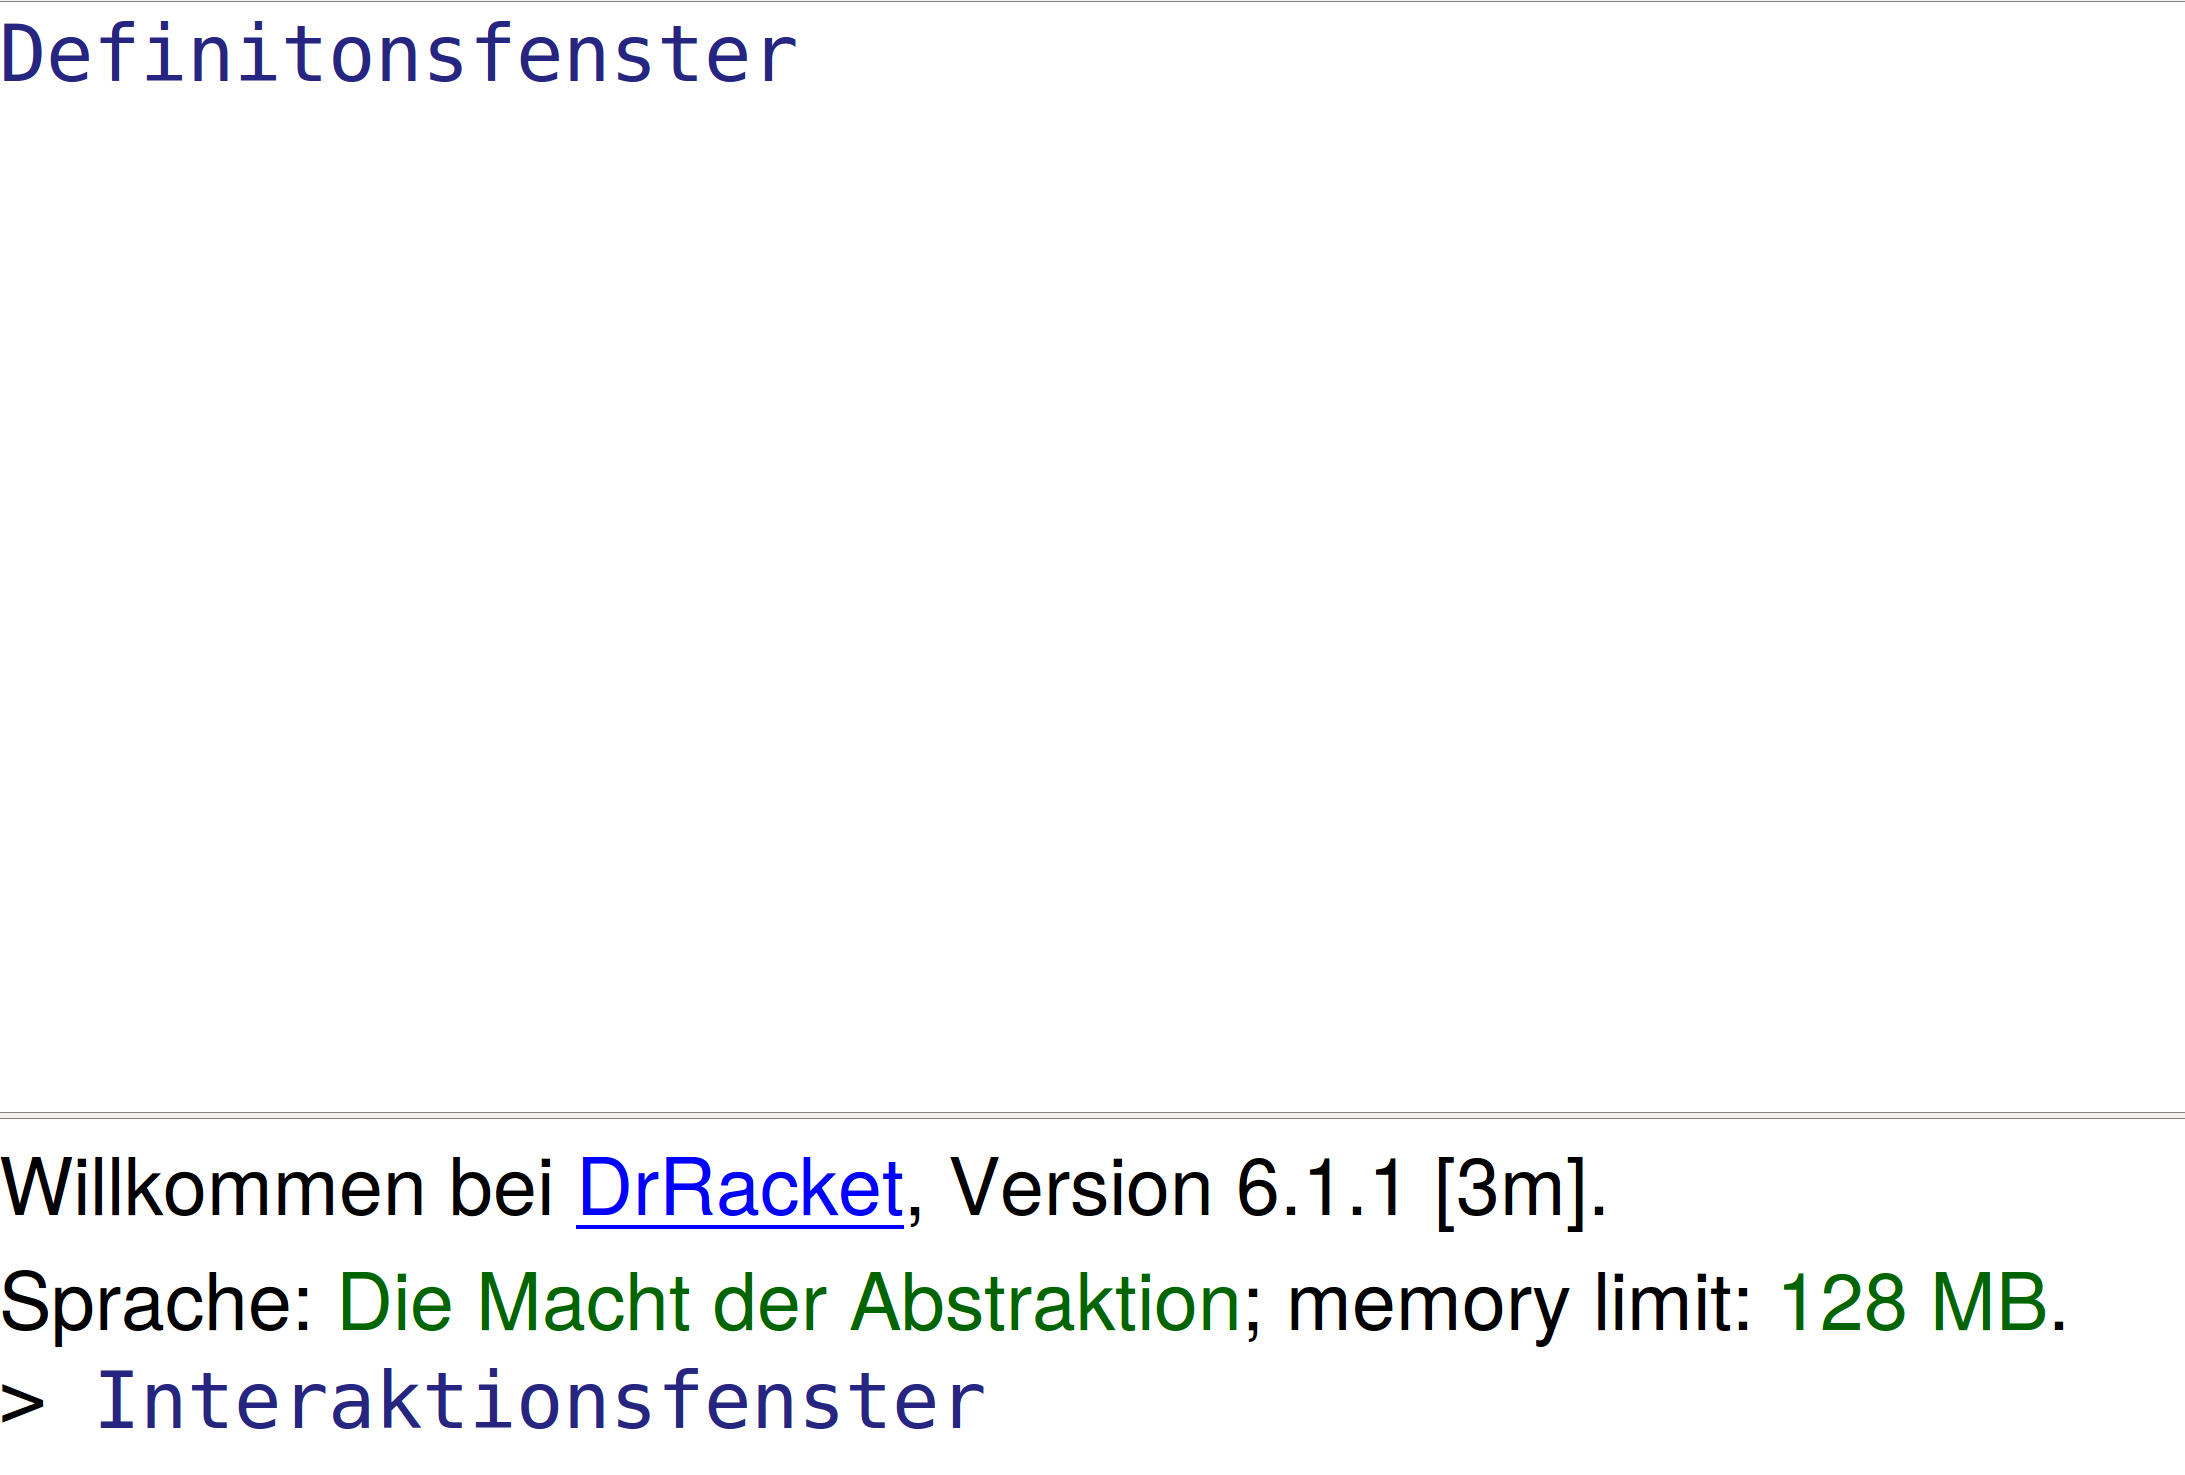
\includegraphics[scale=0.15]{drracket}}\\
Die Anwendung von Funktionen wird in Scheme ausschlie\ss lich in Pr\"afixnotation durchgef\"uhrt
\bigskip\\
\begin{center}
\begin{tabular}{c|c}
Mathematik & Scheme \\
\hline
$44-2$ & \lstinline!(- 44 2)!\\
$f(x,y)$ & \lstinline!(f x y)!\\
$\sqrt{81}$ & \lstinline!(sqrt 81)!\\
$9^2$ & \lstinline!code{(! 3)!\\
\end{tabular}\\
Allgemein: \lstinline[literate=]!(<funktion><argument1><argument2> ...)!
\end{center}
\lstinline!(+ 40 2)! und \lstinline!(odd? 42)! sind Beispiele f\"ur \underline{Ausdr\"ucke}, die bei \underline{Auswertung} einen Wert liefern.\\
(Notation: \eval)\\
\lstinline!(+ 40 2)! $\underbrace{\longrightsquigarrow}_{Reduktion}$ 42\\
\lstinline!(odd? 42)! \eval \ \lstinline!#f!
\bigskip\\
Interaktionsfenster:\hspace*{2.5cm} $\underbrace{Read \rightarrow Eval \rightarrow Print \rightarrow Loop}_{REPL}$\\
\bigskip\\
\underline{Literale} sethen f\"ur einen konstanten Wert (auch: \underline{Konstante}) und sind nicht weiter reduzierbar.\\
\begin{center}
\begin{tabular}{ccc}
Literal &  & Sorte,Typ\\
\hline
\lstinline!#f ,#t! & (true, false, Wahrheitswert) & boolean\\
\lstinline!"x"! & (Zeichenketten) & String\\
\lstinline!0  1904  42  -2 !& (ganze Zahl) & Integer\\
\lstinline!0.42  3.14159 !& (Flie\ss kommazahl) & real\\
\lstinline!1/2, 3/4, -1/10! & (rationale Zahlen) & rational\\

\includegraphics[scale=0.2]{Darth_Vader} & (Bilder) & image

\end{tabular}
\end{center}


